%% This is an example first chapter.  You should put chapter/appendix that you
%% write into a separate file, and add a line \include{yourfilename} to
%% main.tex, where `yourfilename.tex' is the name of the chapter/appendix file.
%% You can process specific files by typing their names in at the 
%% \files=
%% prompt when you run the file main.tex through LaTeX.

\begingroup%
\makeatletter%
\cleardoublepage%
\let\newpage\relax%
\let\clearpage\relax%
\vspace*{\fill}%
\vspace*{\dimexpr-50\p@-\baselineskip}% Remove the initial
%% -default- 50pt gap (plus 1 line) 
\chapter[Preliminary analysis of a microbial community UV exposure experiment at Station ALOHA]{Preliminary analysis of a\\microbial community UV\\exposure experiment at\\Station ALOHA}
\label{AppB}
\vspace*{\fill}%
\endgroup%

\clearpage

\section{Description}

In this appendix, I present some preliminary results from an experiment in which whole, unfiltered surface seawater samples from a site in the North Pacific Subtropical Gyre (NPSG) were exposed to different qualities of natural radiation during a series of shipboard incubations. Samples were analyzed for patterns and biomarkers of lipid photooxidation using the lipidomics pipeline described in \autoref{chap4}.

\section{Brief Summary of Methods}

Seawater was retrieved by CTD from the surface layer at Station ALOHA (22$^{\circ}$ $45'$ N, 158$^{\circ}$ $00'$ W) on 28 March 2016 during cruise KM-1605 aboard the R/V \emph{Kilo Moana}. Approx. 2 L of unfiltered seawater was dispensed using acid-washed tubing into each of 12 acid-washed polyvinyl fluoride (PVF; i.e., Tedlar) air-sampling bags that had modified for oceanographic use with reinforced seals and valves (SKC Inc., Eighty Four, PA, USA). Three \emph{t =} 0 samples were sacrificed immediately. The remaining nine bags containing seawater were then incubated under natural sunlight for 24 hours (from 1600 on 28 March to 1600 on 29 March) in an on-deck aquarium aboard the \emph{Kilo Moana}. Temperature was maintained at 26.2$^{\circ}$C, roughly 1.5$^{\circ}$C warmer than the ambient sea surface temperature. Three light screening treatments were applied (\autoref{fig:abn1}). One set of 3 replicates was incubated without any additional screening, allowing roughly 60 \% of the UVB-range radiation and 75 \% of the UVA-range radiation to reach the sample. A second set of sample bags was shielded during incubation with sheets of 4-mil-thickness polyethylene terephthalate (PET; i.e., Mylar) film, which reduced the dose of UVB radiation reaching the sample to nearly zero (\autoref{fig:abn1}). Finally, three bags were incubated in darkness as a light treatment control. We refer to these treatments as ``+UVB,'' ``-UVB,'' and ``dark control,'' respectively.

Upon sacrificing, 1000 mL of water from each bag was filtered first through a 0.2 $\mu$m pore size Durapore hydrophilic membrane filter (Whatman) to collect particulate phase biomass. The filtrate was passed immediately through a 6 cc Waters Oasis HLB solid-phase extraction (SPE) cartridge containing 200 mg of sorbent (30 $\mu$m particle size; Waters Corporation, Milford, MA, USA). The filters were wrapped in foil and immediately snap-frozen in liquid nitrogen. The SPE cartridges were sealed at both the syringe tip and top opening, wrapped in foil, and frozen immediately at -80$^{\circ}$C. Extraction and HRAM-HPLC-ESI-MS analysis of the particulate samples was performed as described in \autoref{chap3} and \autoref{chap4}. Samples were obtained from the SPE cartridges using a two-phase elution protocol (methanol, followed by acetonitrile) described by Edwards et al. (\emph{in prep}). Both the MeOH and ACN fractions were collected for HRAM-HPLC-ESI-MS analysis. Identification of unoxidized and oxidized lipids was performed according to the methods described in \autoref{chap3} and \autoref{chap4}. Initial feature identification and grouping was performed using xcms (Benton et al., 2010; Smith et al., 2006; Tautenhahn et al., 2008), CAMERA (Kuhl et al., 2012), and LOBSTAHS (Collins et al., 2016); the additional data analysis criteria described in \autoref{chap4} were then applied as an additional means of confirming each lipid identity. IP-DAG and TAG were quantified using authentic standards (Avanti Polar Lipids; Nu-Chek Prep).

\section{Results}

UVB exposure induced changes in both bulk lipid properties and in the relative distributions of individual lipid species within the metalipidome. We positively identified 1,680 individual intact polar diacylglycerol (IP-DAG) and triacylglycerol (TAG) species in particulate samples from the three experimental treatments (\autoref{fig:abn3}b). The fraction of identifiable lipid biomass concentrated in oxidized species was greater in the +UVB treatment after 24 hours of continuous exposure than in either the control or -UVB treatments (compare 47 $\pm$ 35 \% to 27 $\pm$ 6 \% and 28 $\pm$ 9 \%, respectively; mean $\pm$ standard deviation; \autoref{fig:abn2}a). However, the enhanced oxidation we observed in the +UVB treatment was not evenly distributed within the lipid inventory: Membrane lipids (IP-DAG) identified in the +UVB treatment tended to be more oxidized than TAG (compare mole fractions identified as oxidized lipid species of 48 $\pm$ 20 \% and 54 $\pm$~28 \%, respectively; mean $\pm$ standard deviation). Exposure to UVB radiation also significantly reduced the overall size of the lipid inventory in the +UVB treatment compared to the control and -UVB treatment. This effect was highly pronounced, with a reduction of 5666.6 $\pm$ 2827.5 pmol lipid L\textsuperscript{-1} observed in samples from the +UVB treatment (\autoref{fig:abn2}b). An examination of changes in the distributions and abundance of individual lipid species (\autoref{fig:abn3} and \autoref{fig:abn4}) suggested that the increase in lipid oxidation state we observed in the +UVB treatment was due primarily to a disproportionate reduction in the total mass of unoxidized lipid species under prolonged exposure to UVB radiation, and not to a large increase in the mass allocated to oxidized lipids and oxylipins. For example, fluxes of the 25 most abundant lipids in the dataset (nearly all unoxidized) indicate that removal of unoxidized lipids was more significant on a molar basis than production of oxidized lipids (\autoref{fig:abn3}a). However, consistent with the results we observed in liposome experiments (\autoref{chap4}), ingrowth of several oxidized lipid species was observed in the +UVB treatment (\autoref{fig:abn4}). Although these oxidized species did not account for a large fraction of the overall lipid mass, the inventory of species exhibiting the largest relative increase in abundance in the +UVB treatment was dominated by oxidized lipids (\autoref{fig:abn4}).

\clearpage

\section{Figures}

\begin{SCfigure}[0.5][!bh]
\centering
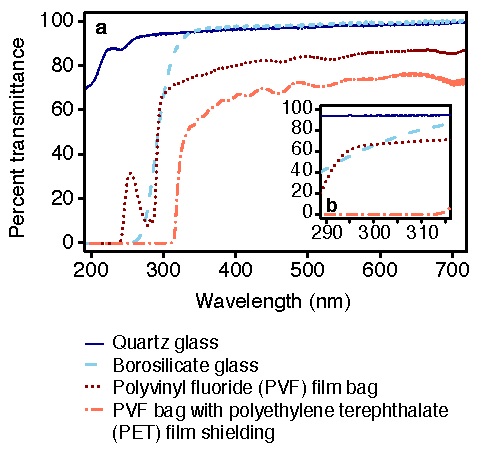
\includegraphics[width=0.6\textwidth]{Fig_B-1.pdf}
\captionsetup{font={footnotesize}}
\caption[Transmission spectra of sampling bags and glass incubation vessels used in lipid photooxidation experiments]{(a) Transmission spectra of the sampling bags and glass incubation vessels used in the lipid photooxidation experiments described in \autoref{AppB} and \autoref{chap4}, respectively. Spectra were measured with a dual-path benchtop spectrophotometer. (b) Inset, showing transmissivities in the UVB spectral band (290-315 nm).}
\label{fig:abn1}
\end{SCfigure}

\clearpage

\begin{figure}[!th]
\centering
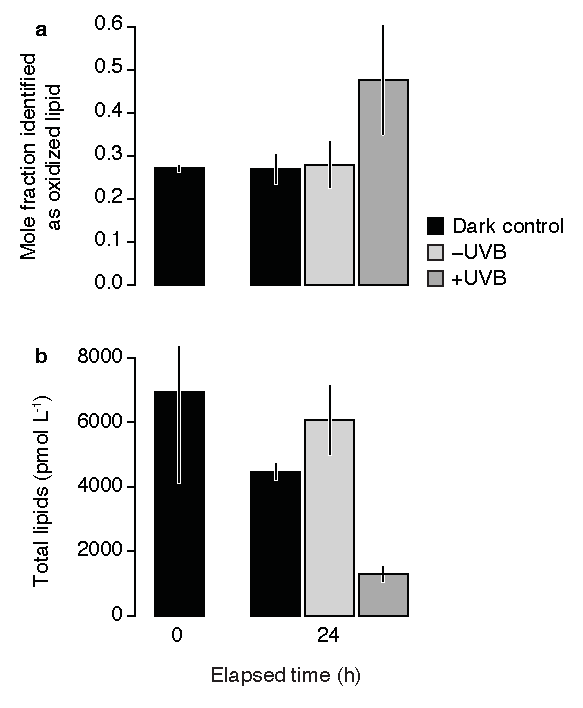
\includegraphics[width=.6\textwidth]{Fig_B-2.pdf}
\captionsetup{font={footnotesize}}
\caption[Bulk properties of lipids over the course of the UV exposure experiment]{Bulk properties of lipids in the particulate fraction over the course of the UV exposure experiment. The two panels show changes in (a) oxidation state and (b) magnitude of the particulate lipid inventory at the two timepoints in the experiment. Results reflect properties of a lipid fraction containing both triacylglycerols (TAGs) and seven classes of intact polar diacylglycerol (IP-DAG). Error bars represent standard errors. In (b), the decrease in lipid concentration observed in the +UVB treatment (-5666.6 $\pm$ 2827.5 pmol lipid L\textsuperscript{-1}) was significant at \emph{p} \textless{} 0.01 using a paired \emph{t-}test, but was not significant (\emph{p} = 0.10) when the difference was evaluated simultaneously with all other possible pairings using Tukey's test for honest significant differences at $\alpha$ = 0.05 (Yandell, 1997)
}
\label{fig:abn2}
\end{figure}

\clearpage

\begin{figure}[!p]
\centering
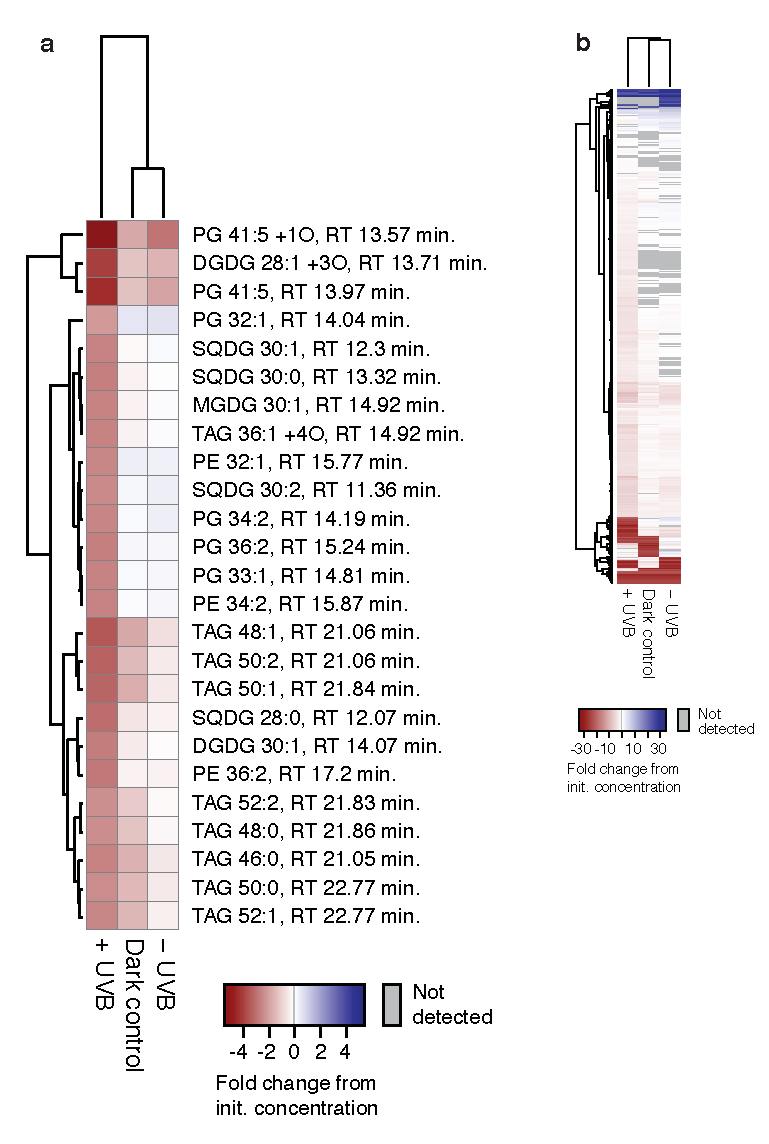
\includegraphics[width=.8\textwidth]{Fig_B-3.pdf}
\end{figure}
\clearpage
\begingroup
\captionsetup{font={footnotesize}}
\captionof{figure}[Changes in individual lipid abundances over the course of the UV exposure experiment]{(preceding page) Changes in individual lipid abundances over the course of the UV exposure experiment. The heatmaps show log\textsubscript{2} (fold) changes after 24 hours in (a) the 25 most abundant individual lipids (TAG or IP-DAG) in the initial, unfiltered seawater sample from Station ALOHA and (b) all positively identified species (\emph{N} = 1680). Dendrogram clustering was performed using an unsupervised clustering algorithm.}
\label{fig:abn3}
\endgroup

\clearpage

\begin{figure}[!p]
\centering
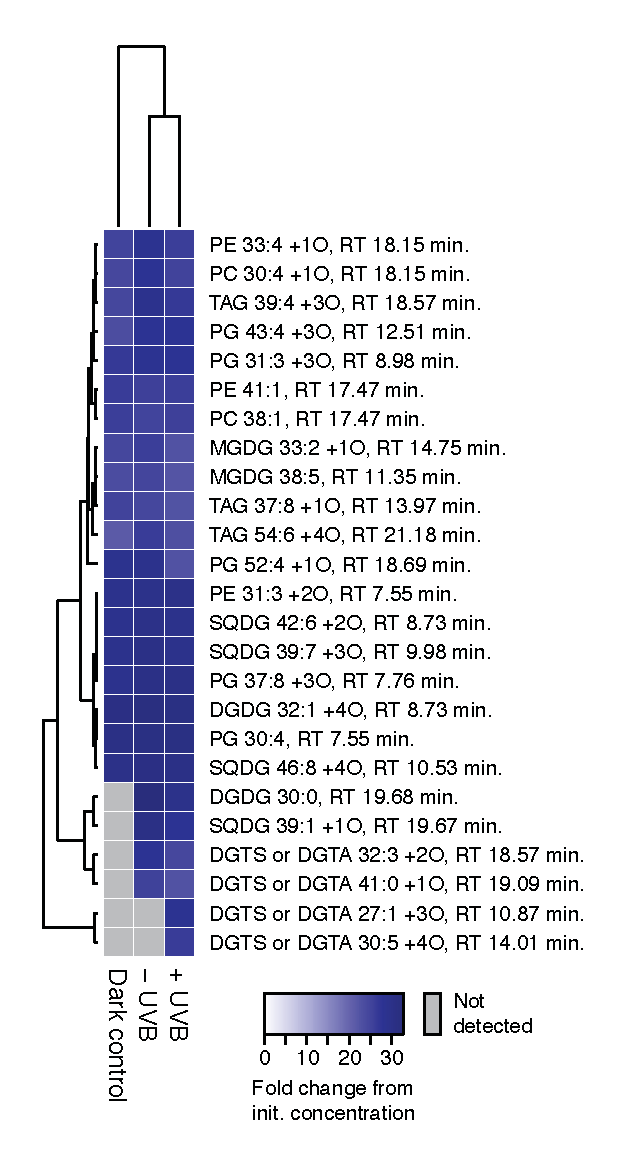
\includegraphics[width=.65\textwidth]{Fig_B-4.pdf}
\end{figure}
\clearpage
\begingroup
\captionsetup{font={footnotesize}}
\captionof{figure}[Log\textsubscript{2} (fold) changes after 24 hours in 25 lipid species]{(preceding page) Log\textsubscript{2} (fold) changes after 24 hours in the 25 lipid species showing the greatest relative increase in the +UVB treatment.}
\label{fig:abn4}
\endgroup

\clearpage

\begin{singlespace}
\section*{References}
\addtocounter{section}{1}
{\setlength{\parindent}{0pt}
Benton, H. P., E. J. Want, and T. M. D. Ebbels (2010), Correction of mass calibration gaps in liquid chromatography-mass spectrometry metabolomics data, \emph{Bioinformatics}, \emph{26}(19), 2488-2489.

{\setlength{\parskip}{10pt}

Collins, J. R., B. R. Edwards, H. F. Fredricks, and B. A. S. Van Mooy (2016), LOBSTAHS: An adduct-based lipidomics strategy for discovery and identification of oxidative stress biomarkers, \emph{Analytical Chemistry}, \emph{88}, 7154-7162, doi:\href{http://dx.doi.org/10.1021/acs.analchem.6b01260}{10.1021/acs.analchem.6b01260}.

Kuhl, C., R. Tautenhahn, C. Bottcher, T. R. Larson, and S. Neumann (2012), CAMERA: an integrated strategy for compound spectra extraction and annotation of liquid chromatography/mass spectrometry data sets, \emph{Analytical Chemistry}, \emph{84}(1), 283-289, doi:\href{http://dx.doi.org/10.1021/ac202450g}{10.1021/ac20245\\0g}.

Smith, C. A., E. J. Want, G. O'Maille, R. Abagyan, and G. Siuzdak (2006), XCMS: processing mass spectrometry data for metabolite profiling using nonlinear peak alignment, matching, and identification, \emph{Analytical Chemistry}, \emph{78}, 779-787.

Tautenhahn, R., C. Boettcher, and S. Neumann (2008), Highly sensitive feature detection for high resolution LC/MS, \emph{BMC Bioinformatics}, \emph{9}, 504.

Yandell, B. S. (1997), \emph{Practical Data Analysis for Designed Experiments}, CRC Press.}}
\end{singlespace}